% ==========================================================================
% ======================== Dokumentace k PC 1.0 ;-) ========================
% ==========================================================================

% Ověřeno, prošlo bez jediné připomínky - při dodržení následujících pokynů:
% - SPRÁVNĚ vyplnit titulní stranu (!!!)
% - Nadpisy používat v pořadí (zanoření):
% 		- chapter (celá kapitola)
%		- section
% 		- subsection, subsubsection ... 
% - Pro pomlčky V TEXTU používat -- (doslova 2 mínusy). Neplatí pro rozsahy
%	(0-9), spojovníky typu xxx-li apod.
% - Uvozovky - používat české \uv{hezké uvozovky}.
% - Zvýrazňovat \textit{kurzívou}.
% - Názvy modulů, funkcí psát \texttt{neproporcionálním fontem}.
% - URL psát do \url{}
% - In-line matematické výrazy přímo do řádky $uzavřené do dolarů$, složitější
%	na samostatnou řádku $$do dvojitých$$.
% - Pokud např. v zadání zmiňujete LATEX a TEX, použít \latex resp. \tex.

% - Pozor na předložky a spojky - nesmí se vyskytovat na konci řádku => použít
%	nedělitelnou mezeru (~).
% - Nové odstavce dvojitým odřádkováním.

% OBRÁZKY	- Vektorově (!!!) - Illustrator, free Inkscape.
% 			- Rastrově vkládat jen screeny obrazovky.
%			- V textu pak odkazovat pomocí \ref{img1}.
%			- Pro úpravu velikosti změnit scale.
% 	\begin{figure}[h]
%		\centering
%		\includegraphics[scale=1.0]{soubor.pdf/png}
%		\caption{Popisek}
%		\label{img1}
%	\end{figure}

% PŘELOŽENÍ
% - Nainstalovat doporučený MiKTeX.
% - "pdflatex <nazev-souboru>.tex"
% - Pro správné vygenerování odkazů, obsahu nutné vždy spustit 2x (!!!)
% - Pro zjednodušení stačí spouštět přibalený bat, který to udělá sám ;)

% ^^^^^^^^^^^^^^^^^^^^^^^^^^^^^^^^^^^^^^^^^^^^^^^^^^^^^^^^^^^^^^^^^^^^^^^^^^
% ^^^^^^^^^^^^^^^^^ !!!!!!!!!SMAZAT PŘI ODEVZDÁNÍ!!!!!!!!! ^^^^^^^^^^^^^^^^^
% ^^^^^^^^^^^^^^^^^^^^^^^^^^^^^^^^^^^^^^^^^^^^^^^^^^^^^^^^^^^^^^^^^^^^^^^^^^

\documentclass[
12pt,
a4paper,
pdftex,
czech,
titlepage
]{report}

\usepackage[czech]{babel}
\usepackage[utf8]{inputenc}
\usepackage{lmodern}
\usepackage{textcomp}
\usepackage[T1]{fontenc}
\usepackage{amsfonts}
\usepackage{titlesec}
\usepackage{graphicx}
\usepackage[hidelinks]{hyperref}
\usepackage{caption}
\usepackage{pdfpages}
\usepackage{xcolor}


\titleformat{\chapter}
  {\normalfont\LARGE\bfseries}{\thechapter}{1em}{}
\titlespacing*{\chapter}{0pt}{0ex plus 1ex minus .2ex}{2.0ex plus .2ex}

\begin{document}

\begin{titlepage}
	\vspace*{-2cm}
	{\centering
\includegraphics[scale=0.5]{FAV_logo_jvs}\par}
	\centering
	\vspace*{2cm}
	{\Large Semestrální práce z KIV/UPA\par}
	\vspace{1.5cm}
	{\Huge\bfseries Návrh automatu\par}
	\vspace{2cm}

	{\Large Petr Laštovka\par}
	{\Large A15B0055K\par}
	{\Large jokertwo@students.zcu.cz\par}

	\vfill

	{\Large 25.\,1.\,2019}
\end{titlepage}

\thispagestyle{empty}
\clearpage


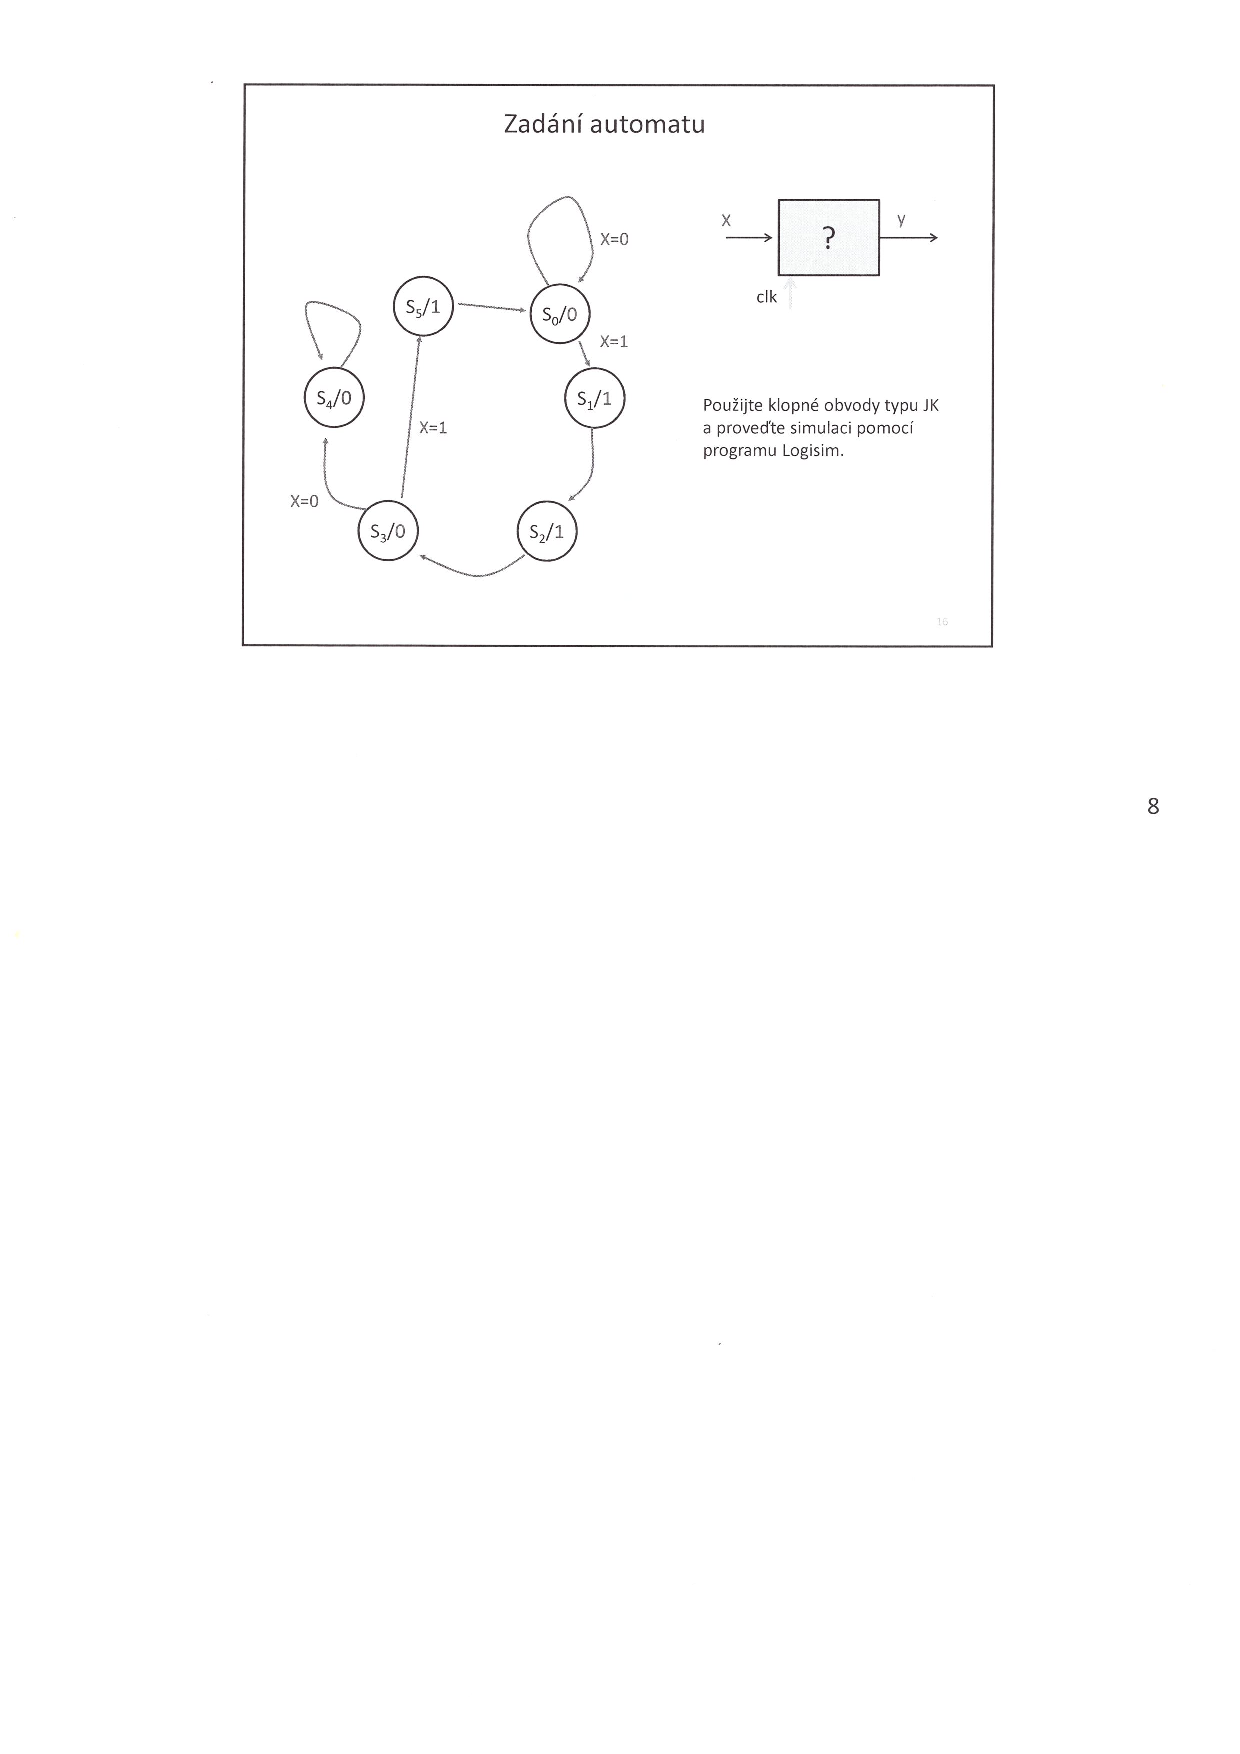
\includepdf[pages=1]{SCAN0001.pdf}


% Table generated by Excel2LaTeX from sheet 'Sheet1'
\section{Tabulky}
\begin{table}[!h]
\begin{minipage}{.5\linewidth}
      \caption{Zápis grafu tabulkou}
      \centering
        \begin{tabular}{l|ccc}
    $S_n$   &  $x=0$  & $x=1$  & \multicolumn{1}{l}{Výstup} \\
    \hline
    $S_0$    & $S_0$    & $S_1$    & 0 \\
    $S_1$    & $S_2$    & $S_2$    & 1 \\
    $S_2$    & $S_3$    & $S_3$    & 1 \\
    $S_3$    & $S_4$    & $S_5$    & 0 \\
    $S_4$    & $S_4$    & $S_4$    & 0 \\
    $S_5$    & $S_0$    & $S_0$    & 1 \\
    \end{tabular}%
    \end{minipage}%
    \begin{minipage}{.5\linewidth}
      \centering
        \caption{Kódování stavů}
         \begin{tabular}{l|rrr}
    $S_n$    & $s_1$ & $s_2$ & $s_3$ \\
        \hline
    $S_0$    & 0     & 0     & 0 \\
    $S_1$   & 0     & 0     & 1 \\
    $S_2$    & 0     & 1     & 0 \\
    $S_3$   & 0     & 1     & 1 \\
    $S_4$   & 1     & 0     & 0 \\
    $S_5$    & 1     & 0     & 1 \\
    \end{tabular}%

    \end{minipage} 

   
  \label{tab:addlabel}%
\end{table}%

% Table generated by Excel2LaTeX from sheet 'Sheet1'
\begin{table}[h]
  \centering
  \caption{Zápis grafu tabulkou se zakódovanými stavy}
    \begin{tabular}{|l|l|l|r|}
    Stav ($s_1 s_2 s_3$) &$x=0$  & $x=1$ & Výstup \\

    000   & 000   & 001   & 0 \\

    001   & 010   & 010   & 1 \\

    010   & 011   & 011   & 1 \\

    011   & 100   & 101   & 0 \\

    100   & 100   & 100   & 0 \\

    101   & 000   & 000   & 1 \\
    \end{tabular}%
  \label{tab:addlabel}%
\end{table}%

\begin{table}[h]
  \centering
  \caption{Budící funkce obvodu JK}
    \begin{tabular}{cccc}
    $Q_s$    & $Q_n$    & J     & K \\
      \hline
    0     & 0     & 0     & x \\
    0     & 1     & 1     & x \\
    1     & 0     & x     & 1 \\
    1     & 1     & x     & 0 \\
    \end{tabular}%
  \label{tab:addlabel}%
\end{table}%

% Table generated by Excel2LaTeX from sheet 'Sheet1'
\begin{table}[h]
  \centering
  \caption{Návrh s JK-klopnými obvody}
    \begin{tabular}{llll|llll|llllll}
    In    &       &       &       & Out   &       &       &       & JK    &       &       &       &       &  \\
    $s_1$    & $s_2$    & $s_3$    & $X$     & $s_1$    & $s_2$    & $s_3$    & $Y$    & $J_1$    & $K_1$    & $J_2$    & $K_2$    & $J_3$    & $K_3$ \\
    \hline
    0     & 0     & 0     & 0     & 0     & 0     & 0     & 0     & 0     & x     & 0     & x     & 0     & x \\
    0     & 0     & 0     & 1     & 0     & 0     & 1     & 0     & 0     & x     & 0     & x     & 1     & x \\
    0     & 0     & 1     & 0     & 0     & 1     & 0     & 1     & 0     & x     & 1     & x     & x     & 1 \\
    0     & 0     & 1     & 1     & 0     & 1     & 0     & 1     & 0     & x     & 1     & x     & x     & 1 \\
    0     & 1     & 0     & 0     & 0     & 1     & 1     & 1     & 0     & x     & x     & 0     & 1     & x \\
    0     & 1     & 0     & 1     & 0     & 1     & 1     & 1     & 0     & x     & x     & 0     & 1     & x \\
    0     & 1     & 1     & 0     & 1     & 0     & 0     & 0     & 1     & x     & x     & 1     & x     & 1 \\
    0     & 1     & 1     & 1     & 1     & 0     & 1     & 0     & 1     & x     & x     & 1     & x     & 0 \\
    1     & 0     & 0     & 0     & 1     & 0     & 0     & 0     & x     & 0     & 0     & x     & 0     & x \\
    1     & 0     & 0     & 1     & 1     & 0     & 0     & 0     & x     & 0     & 0     & x     & 0     & x \\
    1     & 0     & 1     & 0     & 0     & 0     & 0     & 1     & x     & 1     & 0     & x     & x     & 1 \\
    1     & 0     & 1     & 1     & 0     & 0     & 0     & 1     & x     & 1     & 0     & x     & x     & 1 \\
    \end{tabular}%
  \label{tab:addlabel}%
\end{table}%

\begin{table}[!h]
\begin{minipage}{.5\linewidth}
      \caption{Karnaughova mapa\\ pro Y}
      \centering
    \begin{tabular}{lllllll}
      			       &       					 &       				 & &	\colorbox{yellow}{}& \colorbox{yellow}{}         &$s_1$ \\
    		 	       &        					&        & \colorbox{red}{}    & \colorbox{red}{}				      &         &$s_2$     \\
    		 	       &        					& 0    				 & 1    				   & x     				& 0       &  \\
              	       & \colorbox{black}{}       & 0     				 & 1    				   & x   		  			& 0       &  \\
\colorbox{blue}{}& \colorbox{black}{}       & 1    				 & 0     				   & x     				& 1       &  \\
\colorbox{blue}{}&       					 & 1   				 & 0				  	   & x    					& 1       &  \\
    	  $ s_3$ 	& $x$  					&     				 &       				   &       				  	 &          &  \\
    \end{tabular}%
  \end{minipage}%
    \begin{minipage}{.5\linewidth}
      \centering
        \caption{Karnaughova mapa\\ pro $J_1$}
    \begin{tabular}{lllllll}
      			       &       					 &       				 &  &	\colorbox{yellow}{}&  \colorbox{yellow}{}       &$s_1$ \\
    		 	       &        					&        & \colorbox{red}{}    & \colorbox{red}{}				      &         &$s_2$     \\
    		 	       &        					& 0    				 & 0    				   & x     				& x       &  \\
              	       & \colorbox{black}{}       & 0     				 & 0    				   & x   		  			& x       &  \\
\colorbox{blue}{}& \colorbox{black}{}       & 0    				 & 1     				   & x     				& x       &  \\
\colorbox{blue}{}&       					 & 0   				 & 1				  	   & x    					& x       &  \\
    	  $ s_3$ 	& $x$  					&     				 &       				   &       				  	 &          &  \\
    \end{tabular}%
  \end{minipage} 

   
  \label{tab:addlabel}%
\end{table}%

\newpage 
\begin{table}[!h]
\begin{minipage}{.5\linewidth}
      \caption{Karnaughova mapa\\ pro $K_1$}
      \centering
    \begin{tabular}{lllllll}
      			       &       					 &       				 &  &	\colorbox{yellow}{}& \colorbox{yellow}{}        &$s_1$ \\
    		 	       &        					&       & \colorbox{red}{}    & 	\colorbox{red}{} 			      &         &$s_2$     \\
    		 	       &        					& x   				 & x    				   & x     				& 0       &  \\
              	       & \colorbox{black}{}       & x     				 & x    				   & x   		  			& 0       &  \\
\colorbox{blue}{}& \colorbox{black}{}       & x    				 & x     				   & x     				& 1       &  \\
\colorbox{blue}{}&       					 & x   				 & x				  	   & x    					& 1       &  \\
    	  $ s_3$ 	& $x$  					&     				 &       				   &       				  	 &          &  \\
    \end{tabular}%
  \end{minipage}%
    \begin{minipage}{.5\linewidth}
      \centering
        \caption{Karnaughova mapa\\ pro $J_2$}
    \begin{tabular}{lllllll}
      			       &       					 &       				 &  &	\colorbox{yellow}{}&\colorbox{yellow}{}         &$s_1$ \\
    		 	       &        					&      & \colorbox{red}{}    & 	\colorbox{red}{}  			      &         &$s_2$     \\
    		 	       &        					& 0    				 & x    				   & x     				& 0       &  \\
              	       & \colorbox{black}{}       & 0     				 & x    				   & x   		  			& 0       &  \\
\colorbox{blue}{}& \colorbox{black}{}       & 1    				 & x     				   & x     				& 0       &  \\
\colorbox{blue}{}&       					 & 1   				 & x				  	   & x    					& 0       &  \\
    	  $ s_3$ 	& $x$  					&     				 &       				   &       				  	 &          &  \\
    \end{tabular}%
  \end{minipage} 

   
  \label{tab:addlabel}%
\end{table}%

\newpage 
\begin{table}[!h]
\begin{minipage}{.5\linewidth}
      \caption{Karnaughova mapa\\ pro $K_2$}
      \centering
    \begin{tabular}{lllllll}
      			       &       					 &       				 &  &	\colorbox{yellow}{}& \colorbox{yellow}{}        &$s_1$ \\
    		 	       &        					&       & \colorbox{red}{}    & 	\colorbox{red}{} 			      &         &$s_2$     \\
    		 	       &        					& x   				 & 0    				   & x     				& x       &  \\
              	       & \colorbox{black}{}       & x     				 & 0    				   & x   		  			& x       &  \\
\colorbox{blue}{}& \colorbox{black}{}       & x    				 & 1     				   & x     				& x       &  \\
\colorbox{blue}{}&       					 & x   				 & 1				  	   & x    					& x       &  \\
    	  $ s_3$ 	& $x$  					&     				 &       				   &       				  	 &          &  \\
    \end{tabular}%
  \end{minipage}%
    \begin{minipage}{.5\linewidth}
      \centering
        \caption{Karnaughova mapa\\ pro $J_3$}
    \begin{tabular}{lllllll}
      			       &       					 &       				 &  &	\colorbox{yellow}{}&   \colorbox{yellow}{}     &$s_1$ \\
    		 	       &        					&       & \colorbox{red}{}    & 		\colorbox{red}{} 		      &         &$s_2$     \\
    		 	       &        					& 0    				 & 1    				   & x     				& 0       &  \\
              	       & \colorbox{black}{}       & 1     				 & 1    				   & x   		  			& 0       &  \\
\colorbox{blue}{}& \colorbox{black}{}       & x    				 & x     				   & x     				& x       &  \\
\colorbox{blue}{}&       					 & x   				 & x				  	   & x    					& x       &  \\
    	  $ s_3$ 	& $x$  					&     				 &       				   &       				  	 &          &  \\
    \end{tabular}%
  \end{minipage} 

   
  \label{tab:addlabel}%
\end{table}%

\begin{table}[!h]
 \centering
        \caption{Karnaughova mapa\\ pro $K_3$}
    \begin{tabular}{lllllll}
      			       &       					 &       				 & 						 &	\colorbox{yellow}{}& \colorbox{yellow}{}	        &$s_1$ \\
    		 	       &        					&        & \colorbox{red}{}    & 	\colorbox{red}{}			      &         &$s_2$     \\
    		 	       &        					& x    				 & x    				   & x     				& x       &  \\
              	       & \colorbox{black}{}       & x     				 & x    				   & x   		  			& x       &  \\
\colorbox{blue}{}& \colorbox{black}{}       & 1    				 & 0     				   & x     				& 1       &  \\
\colorbox{blue}{}&       					 & 1   				 & 1				  	   & x    					& 1       &  \\
    	  $ s_3$ 	& $x$  					&     				 &       				   &       				  	 &          &  \\
    \end{tabular}%
\end{table}%
\pagebreak	
\newpage
\newpage


Výrazy po zjednodušení':
\begin{itemize}
\item $y = (\neg s_1 \lor s_2) \land (\neg s_3 \lor s_2)$
\item $J_1 = s_2 \lor s_3$
\item $K_1 = s_3$
\item $J_2 = \neg s_1 \lor s_3$
\item $K_2 = J_2$
\item $J_3 = (\neg s_1 \lor s_2) \land (\neg s_1 \lor \neg s_3 \lor x)$
\item $K_3 = (\neg s_2 \lor s_3) \land (s_3 \lor \neg s_1 \lor \neg x)$
\end{itemize}

	

\begin{figure}[h]
	\centering
	
		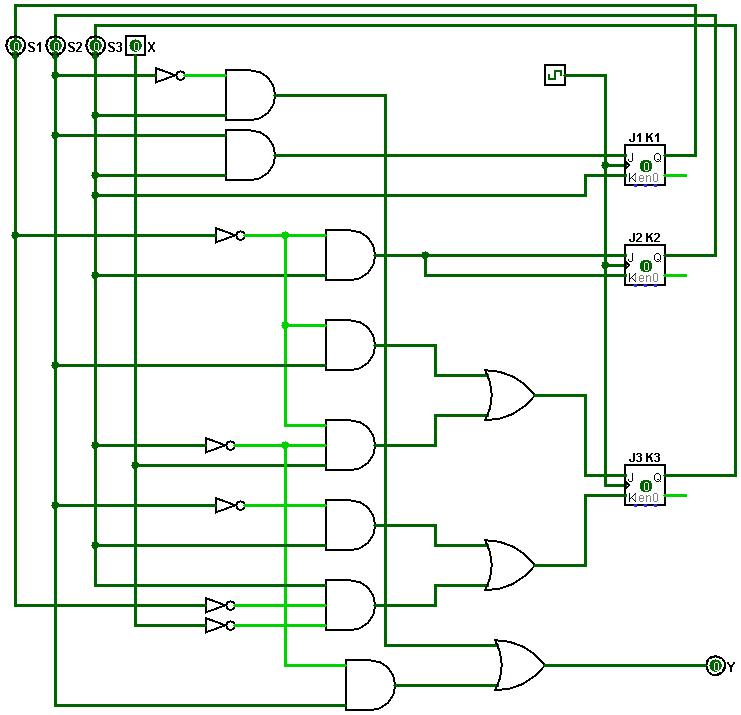
\includegraphics[scale=.5]{automat.jpg}
		\caption{Návrh logického automatu}
		\label{fig:klient01}
	\end{figure} 
	
	
\end{document} 